\documentclass{article}
\usepackage[T2A]{fontenc}
\usepackage[utf8x]{inputenc}
\usepackage[english]{babel}
\usepackage{float}
\usepackage{graphicx}
\usepackage{hyperref}
\usepackage{cleveref}
\usepackage{xcolor}
\usepackage{subcaption}
\usepackage{listings}
\usepackage{tabularx}

% \def\mybibname{\fontencoding{T2A}\selectfont
% \CYRL\cyri\cyrt\cyre\cyrr\cyra\cyrt\cyru\cyrr\cyra}
% \def\myshortname{%%%
% \fontencoding{T2A}\selectfont
%   \CYRM\cyro\cyrd\cyre\cyrl.
%   \cyri{}
%   \cyra\cyrn\cyra\cyrl\cyri\cyrz{}
%   \cyri\cyrn\cyrf\cyro\cyrr\cyrm.
%   \cyrs\cyri\cyrs\cyrt\cyre\cyrm.{}
% }
% \def\mylongname{%%%
% \fontencoding{T2A}\selectfont
%   \CYRM\cyro\cyrd\cyre\cyrl\cyri\cyrr\cyro\cyrv\cyra\cyrn\cyri\cyre{}
%   \cyri{}
%   \cyra\cyrn\cyra\cyrl\cyri\cyrz{}
%   \cyri\cyrn\cyrf\cyro\cyrr\cyrm\cyra\cyrc\cyri\cyro\cyrn\cyrn\cyrery\cyrh{}
%   \cyrs\cyri\cyrs\cyrt\cyre\cyrm{}
% }
% \def\myrecname{\fontencoding{T2A}\selectfont
% \cyrp\cyro\cyrl\cyru\cyrch\cyre\cyrn\cyra}
% \def\myvolname{\fontencoding{T2A}\selectfont
% \CYRT.}
% \def\myUDCname{\fontencoding{T2A}\selectfont
% \CYRU\CYRD\CYRK}
\hypersetup{
    colorlinks,
    linkcolor={black!50!black},
    citecolor={blue!50!black},
    urlcolor={blue!80!black}
}
% Default fixed font does not support bold face
\DeclareFixedFont{\ttb}{T1}{txtt}{bx}{n}{8} % for bold
\DeclareFixedFont{\ttm}{T1}{txtt}{m}{n}{8}  % for normal
\usepackage{color}
\definecolor{deepblue}{rgb}{0,0,0.5}
\definecolor{deepred}{rgb}{0.6,0,0}
\definecolor{deepgreen}{rgb}{0,0.5,0}

% Python style for highlighting
\newcommand\pythonstyle{\lstset{
language=Python,
basicstyle=\ttm,
otherkeywords={self},             % Add keywords here
keywordstyle=\ttb\color{deepblue},
emph={MyClass,__init__},          % Custom highlighting
emphstyle=\ttb\color{deepred},    % Custom highlighting style
stringstyle=\color{deepgreen},
frame=tb,                         % Any extra options here
showstringspaces=false            % 
}}
% Python environment
\lstnewenvironment{python}[1][]
{
\pythonstyle
\lstset{#1}
}
{}

% Python for external files
\newcommand\pythonexternal[2][]{{
\pythonstyle
\lstinputlisting[#1]{#2}}}

% Python for inline
\newcommand\pythoninline[1]{{\pythonstyle\lstinline!#1!}}



\title{Visualizing fakenews as reported by euvsdisinfo.eu}
\author{Jesper Henrichsen \\{\small Supervised by: Pedro Ferreira}}
\begin{document}
\maketitle
\newpage
\tableofcontents
\listoffigures
\newpage

%%%%
% Some title section: A visualization of fakenews reported by euvsdisinfo.eu
%%%%
\section{Introduction}
Misinformation, and in turn: {\it fakenews}, is not a new phenomenon, on the contrary, it far predates modern day in the information age with social media and an ingrained expectation of internet access independent of time and place. Even a sense of a printed distribution of misinformation dates as far back as the 18{\it th} century where, in London, the printed newspapers would publish snippets with stories from questionable sources \cite{first_propaganda}. The same article provides an insight into how compromising information already then had political impact and played a part in the public support for the execution of the queen of France, Marie Antoinette. This was inspite the fact that it was not possible to publish news of the sort avaiable in London, so snippets were left on benches in the parks of Paris \cite{first_propaganda}.
\\\\
Since the introduction of the internet, information has been able to reach further and faster than ever before. Recent developments of omnipresent social media has created the perfect platform for the spread of this information within the internet. In 2016, 62\% of americans received their news from social media \cite{gottfried2016news}. For the sake of advertisement social media platforms has, since their introduction, only become better at targeting their audience with information that will capture their attention. As put by the team behind the newsfeed at Facebook: ``{\it The goal of News Feed is to deliver the right content to the right people at the right time (...)}''\footnote{See: \url{https://www.facebook.com/business/news/News-Feed-FYI-A-Window-Into-News-Feed}}. However, a relevant question would be to whom it is implied to be {\it right} for. That it is not necessarily the user, has recently emerged as a likely answer.
\\\\
The nature of social media has proved to be an effective way for the spread of information, genuine as well as fake.\\
This report will describe the process of scraping and visualizing information from \href{https://euvsdisinfo.eu}{euvsdisinfo.eu}, an EU run campaign that debunks pro Kremlin news stories. One objective of this project was to investigate whether these cases could be used to view fakenews as attacks. And if so, could there be identified a perpetrator either as an outlet or country, and a victim such as the country being mentioned in the information.

\section{Background}
% What and when...
The concept of {\it fakenews} is not a new invention. The term emerged on the public conscious especially during the 2016 american presidential election, where it was mostly used as a deflection of criticism. However, the underlying properties of the recent years fakenews stories are heavily influenced by authentic, mainstream journalism. Some of these properties, in the form of sensationalism which is a type of exaggeration for the purpose of further circulation, occured already in american press in the late 19{\it th} century and was refferred to as {\it yellow journalism} \cite{spencer2007yellow}. The yellow journalism brought about sensationalism and eyecatching headlines which in todays digital world is equivalent to what is commonly denoted as {\it clickbait} titles. Also, just as yellow journalism was about monetizing on circulation, so is much of the fakenews today, but perhaps with the distinction that today, anyone can become the publisher. To exemplify this, a Macedonian village was traced as the origin of many fakenews websites that appeared during the 2016 american election, the incentive was to profit on the generated traffic through advertisement \cite{bbc_mcdVillage}. \\
The notion of clickbait refers to articles with titles that leaves a cliff hanger in order to lure the reader to follow a link to the outlet that hosts the article. Therefore, titles are as important as ever for the circulation since content sharing on socialmedia often only leaves limited space to include relevant information. That fakenews has been successful in terms of exploiting the properties necessary for circulation on social media is highlighted by the fact that the most popular fakenews stories were shared more than the most popular mainstream news stories \cite{allcott2017social}. The fact that socialmedia targets their content towards the endusers individually tends to accellerate the sharing of certain news more rapidly than ever before. This targeting of content also has the effect of creating so called {\it filter bubbles} for the end-user, where they do not see an evenly distributed sample of the content available, but rather a predefined subset that by socialmedia platforms is deemed more likeable for the users to engage with. 
% Why and who...
% the economy behind it...
\\\\
Despite a common claim to oppose fakenews, a consensus of when a story can be labelled as fake is diffuclt to distill. Largely because the term itself has become part of a tactical repetoire for deflecting unwanted criticism. Though more importantly is the inherent opposing interests that gave birth to the stories in the first place. \\ Hunt and Matthew suggests that from an economical perspective fakenews materialize from an equilibrium between producers and readers. The fakenews is much cheaper to provide rather than authentic news. While for the reader it is not costless to deduct inaccuracies, and the reader might even enjoy the partisan news \cite{allcott2017social}. The last part consequently means that the fakenews provides utility for the reader, though at the cost of providing the reader with a false state of the world.
\\\\
Therefore, as the fakenews is hard to distinguish from authentic news as illustrated by {\it A field guide to fakenews} \cite{field_guide_fakenews}, the challenge arises to combat the false information. In Europe the experience in later years has been dominated by a narrative battle that has especially unfolded over the Ukranian conflict \cite{khaldarova2016fake}. This presents a reason for the existence of fakenews articles different from the objective of monetizing on circulation through ads. The fight for a narrative through information spread online, is reminscent of traditional propaganda, with the obvious exception that it utilizes modern technologies.\\
Although fakenews might pose a threat to the common empirical foundation that is implicitly assumed by a democratic society, the multifaceted properties of fakenews makes it a difficult problem to approach \cite{the_economist}. For this reason, there exists many initiatives that seeks to debunk the false information.
Examples of such are the privately run fact-checking website, \url{http://snopes.com}, which historically has focused on debunking or validating urban legends. Another site is the ukrainian fact-checking site: \url{http://stopfake.org}, a domain bought in 2014\footnote{See {\texttt whois}: \url{https://whois.icann.org/en/lookup?name=stopfake.org}}.
\\\\
This report focuses on the debunked cases provided by \href{https://www.euvsdisinfo.eu}{euvsdisinfo.eu}, even though both of the fact checking websites listed above has existed for longer. The reasoning for this choice, is that for the purpose of this project, the \href{https://www.euvsdisinfo.eu}{euvsdisinfo.eu} was sufficient as it provided access to a wide variety of cases in a structured way. At the same time it is an interesting aspect that the repository is maintained as an EU funded campaign.
%The reasoning for this choice, is that the campaign website with its listed cases, provides an structured accessible resource for investigation of whether such repositories could be used for automising visualizations to interpret the state of news it contains. % living on the edge, possibly reformulate.. make sure this is fucking in line! 
\\
The campaign has existed since 2015 and is run by the European External Action Service East Stratcom Task Force. The primary focus of the campaign is to identify and debunk pro-Kremlin disinformation.
The campaign includes cases of debunked information from sources spanning from official news sites to twitter accounts, to non-online content such as interviews. The website \href{https://www.euvsdisinfo.eu}{euvsdisinfo.eu} includes, at the time of writing, more than 3400 such cases, these are the cases that this report is based on. The cases are all reported either by the campaign staff themselves, or one of the 400 collaborating organizations and individuals.
In \cref{fig:cases} is seen how cases are listed on the website, the order of which is chronological with respect to the date it was reported.

\begin{figure}[H]
    \centering
    \caption{Example listing of disinformation cases on \href{https://www.euvsdisinfo.eu}{euvsdisinfo.eu}}
    \label{fig:cases}
    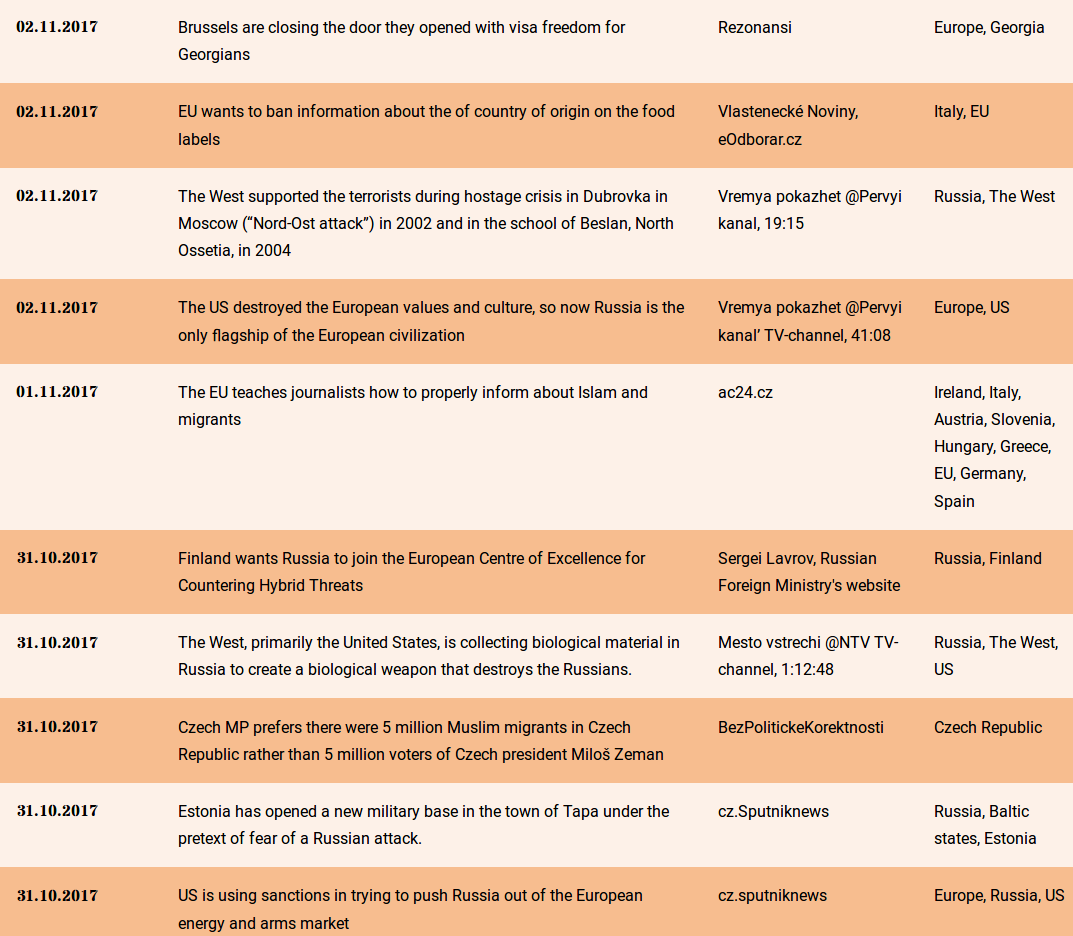
\includegraphics[width=.9\textwidth]{images/example_cases.png}
\end{figure}

As seen by \cref{fig:cases}, the cases are listed showing the date they were reported, an english title to the story, a name of an outlet that published the story, and a country of origin. 

\section{Acquiring a dataset}
In this section, the approach to acquiring and extracting information for visualization will be described. The initial dataset was scraped from \href{https://www.euvsdisinfo.eu}{euvsdisinfo.eu}, however, this dataset was gradually extended in a number of steps. These steps will be described in this section.

\subsection{Scraping the cases}
The cases listed at \href{https://www.euvsdisinfo.eu}{euvsdisinfo.eu} consists of information regarding the case, such as who reported it, in what country or countries did it originate in, as well as the disproof that debunks the information as invalid. Other information for each case is meta information about the information and its source. In \cref{fig:single_case} is seen an example of the information listed for a specific case.
\begin{figure}[H]
    % \begin{subfigure}[b]{.3\textwidth}
    \centering
    \caption{An example of the information for each case}
    \label{fig:single_case}
    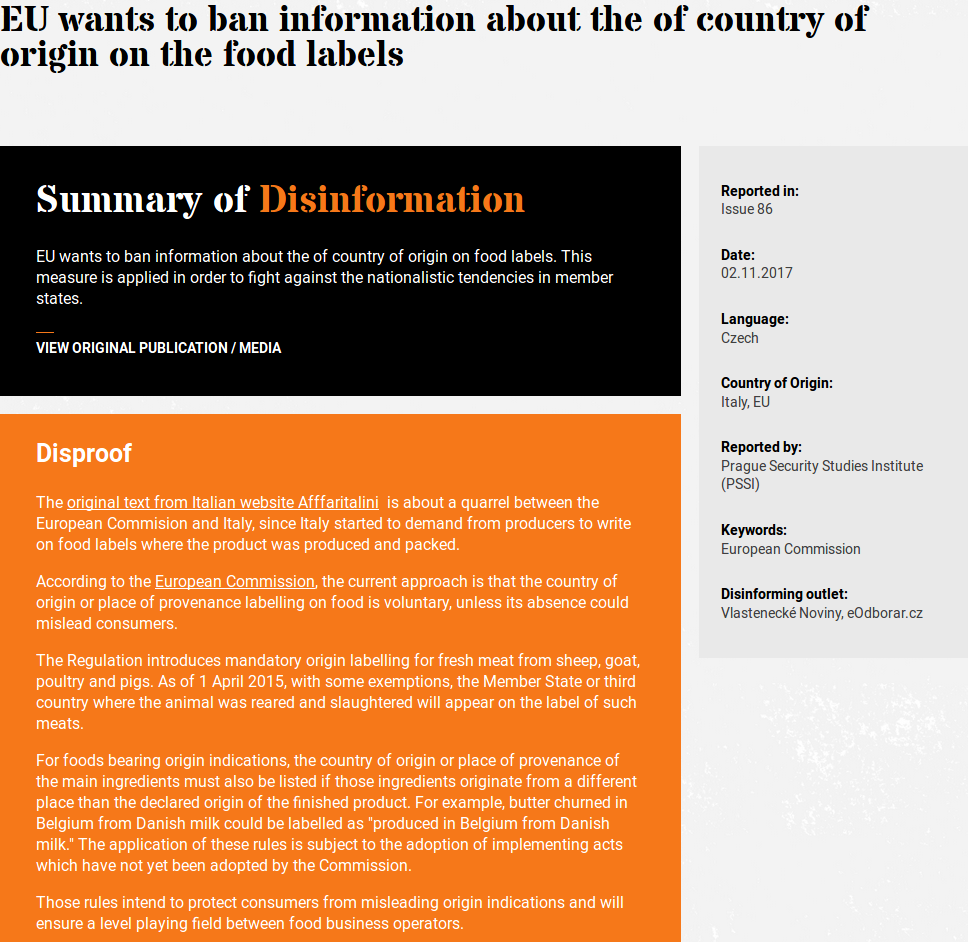
\includegraphics[width=.9\textwidth]{images/example_fakenews.png}
    % \end{subfigure}%
\end{figure}
There is no API, or otherwise download button on the campaign website to get the whole dataset as is. However, there is no mention in their {\texttt robots.txt} file that indicates that scraping is not permitted. Therefore, the intial dataset was achieved after writing a scraper in Python\footnote{\url{https://github.itu.dk/jeshe/fakenews-scraper/blob/master/news_scraper.py}}. The list of cases is an overview list with a pagination of $10$ cases per page, an example of this list is shown in \cref{fig:cases}. The offset is given by the URL, and so the crawling to acquire links to each specific page can be done in a well defined way, without having to worry about the specific structure of the website.
However, parsing of the structure of the website is necessary in order to scrape the information of each specific case. For this, the python library {\texttt BeautifulSoup}\footnote{\url{https://www.crummy.com/software/BeautifulSoup/}} was heavily used.\\
In the end, the information was saved into a csv file containing one disinformation case per row, and in total $3071$ data rows.

\subsection{Article scraping and content extraction}
In order to get more information than was already available for each case at \url{euvsdisinfo}, information from the original source was also included and added to the dataset. This section will describe the approach that was used in order to reliably get information across the many differently structured websites.
\\\\

\begin{figure}[H]
    % \begin{subfigure}[b]{.3\textwidth}
    \centering
    \caption{An example of a debunked news article from a Czech website}
    % \caption{An example of an original article from a Czech website that was debunked as  }
    \label{fig:fake_source}
    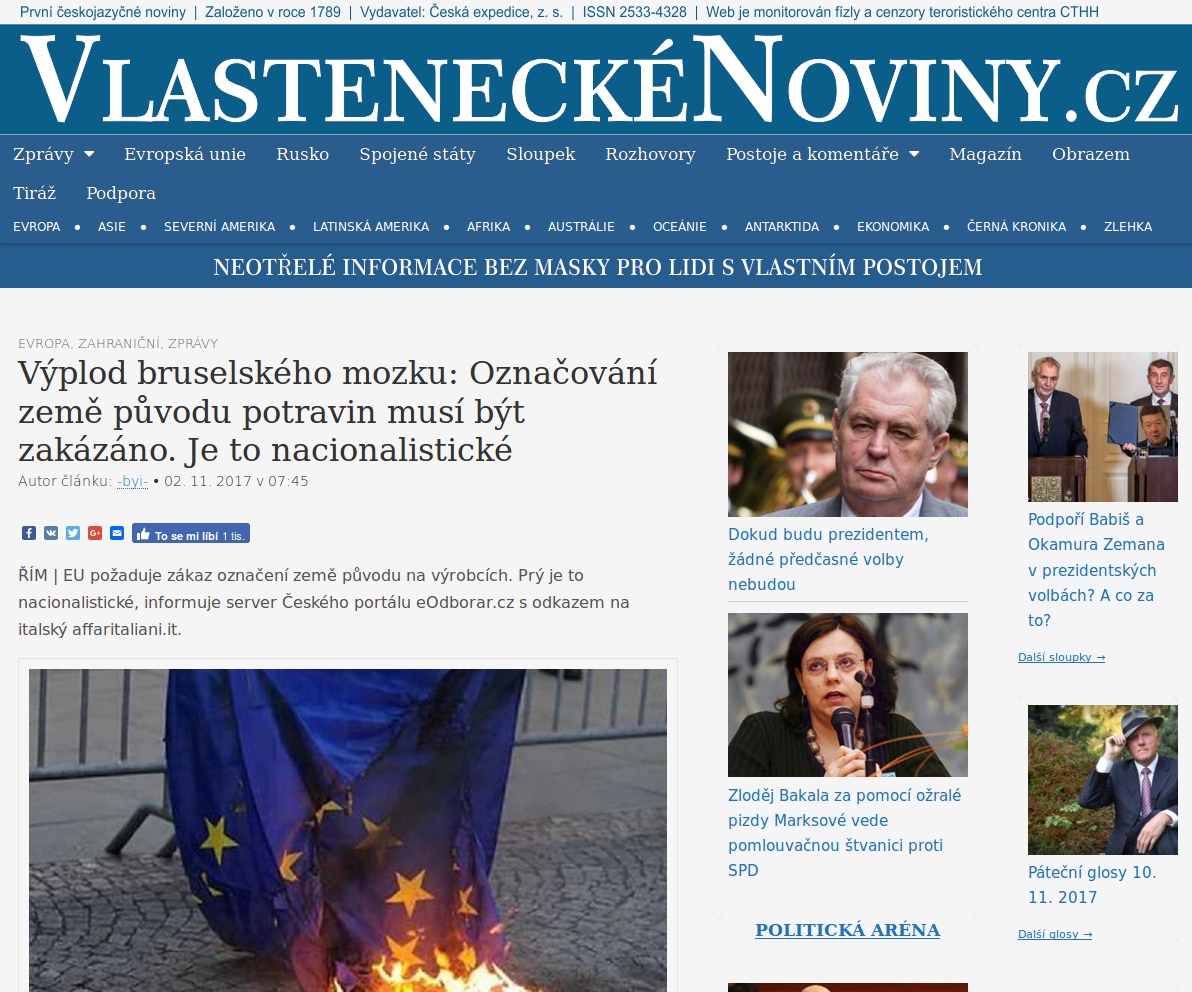
\includegraphics[width=.9\textwidth]{images/example_source.png}
    % \end{subfigure}
\end{figure}
A general approach to extracting content is difficult because source of information can be any sort of media, whether digital or physical, in writing or a video. And, because each website is different, then even building a scraper to extract the content of the subset of sources that are online articles, will be difficult. In \cref{fig:fake_source} is seen an example of a source article.
\\
One important property for the purpose of this project is that in order to consider the names of locations that are being mentioned in the articles, the entire content is not strictly necessary. Therefore, I chose to use the meta tags to extract information about the content, summary, titles, author, and descriptions of each online resource.
I would also filter on html tags such as the header tags, {\texttt h1}, {\texttt h2}, {\texttt h3}, {\texttt h4}, {\texttt h5}, {\texttt h6} as well as the {\texttt title} tag used for setting the window title. I found through experiment that only considering the first occuring header tag worked best, the reason is that other header tags than the first one would often be titles of other news articles that the news site wants the user to click on.
% \\\\
\begin{figure}[H]
\caption{Meta tags defined in python scraper}
\label{fig:python_metatags}
\begin{python}
metatag_list = [
    ("name", "description", "content"),
    ("property" "og:title", "content"),
    ("property", "og:description", "content"),
    ("name", "twitter:title", "content"),
    ("name", "twitter:description", "content"),
    ("name", "language", "content"),
    ("name", "keywords", "content"),
    ("name", "subject", "content"),
    ("name", "topic", "content"),
    ("name", "summary", "content"),
    ("name", "subtitle", "content"),
    ("itemprop", "name", "content"),
    ("itemprop", "description", "content"),
]
tag_list = [ ("h%s" % i, None) for i in range(1, 7) ] + [("title", None)]
\end{python}
\end{figure}

Extracting content by meta tags proved to be a very reliable approach, since most news sites are interested in their content being shared. So, in order to optimize sharability almost all online resources had optimized for search engines, often reffered as just: {\it SEO}. In \cref{fig:python_metatags} is seen the defined metatags that the scraper was looking for, defined in the variable: {\texttt metatag\_list}, as well as the list of header and title tags defined in {\texttt tag\_list}. Each metatag is defined as a tripplet. The first value defines what attribute to look for when finding a HTML tag of type {\texttt meta}, the second what value such attribute should have. When a match is found for the first two, then the third string in the tripple is used to know from what attribute to extract text from. In the metatags listed in \cref{fig:python_metatags} all content was extracted from attributes of the same name regardless of the match on the first two. However, defining triples makes this method generalize to any other metatags that might be relevant to add in the future. The reasoning behind the list of other HTML tags being defined as tuples, is similar. Although, for my purposes, the second string was set to {\texttt None}, in which case the script would scrape the inner HTML of the element instead of the content of a named attribute.
\\\\
In order to avoid duplicating content as much as possible the content of a meta tag or html tag was compared to the content that was already found in previous tags. This approach resulted most often in a short paragraph of information about the article, including keywords, title and summary. Before applying the approach to the articles scraped from \href{https://www.euvsdisinfo.eu}{euvsdisinfo.eu}, it was tested on arbitrarily chosen articles, such as articles from danish news outlets. It was also tried on a sample of articles taken from the subreddits: r/politics, r/news, and {r/worldnews}\footnote{\url{https://reddit.com/r/politics+news+worldnews}}, because these were collections of news articles with a good variety of news outlets. The results were used to evaluate qualitatively on the smaller sample. None of which turned out to have no content, and only one resulted in an extract only consisting of keywords. Interestingly, among the keywords for that particular result were also the name of the country that the news story revolved around. \\
One thing that was clear from this, was that locations were not always mentioned if the news concerned well known state leaders such as Putin, Merkel or Trump. In such cases, often only the names of the state leaders were present as indication of what countries were mentioned in the articles.

\subsection{Named entity recognition}
One initially desired outcome was the possibility to extract location information about what countries were being mentioned in the articles. This section will describe the approach to using stanford NER tagger to quantitatively extract location names from the meta information acquired for each article.
\\\\
Named entity recognition is a research field within natural language processing concerned with recognizing names of things such as people, company names, or, as relevant for this project, locations. The study of recognizing location names within texts is one of the most studied areas of named entity recognition, however, still an ongoing research. As such the NER tagger used in this project is released open source as part of the Stanford nlp library\cite{manning-EtAl:2014:P14-5} which also includes many other models and methods relevant to the field of natural language processing. 
%The NER tagger used for this project was a pretrained model trained on a corpus of both e [motherfucking reference] 
A more in depth explanation of named entity recognition or even natural language processing, is however, beyond the scope of this project. 
%Instead for the purposes of this project, I will rely on existing tools.
In \cref{fig:ner_tagging} is seen an example of tagging a sentence using the graphical interface of the NER tagger. The sentence in \cref{fig:ner_tagging} is arbitrarily chosen from Wikipedia, and is not part of the content of the dataset.

\begin{figure}[H]
\caption{NER tagging on a sample sentence}
\label{fig:ner_tagging}
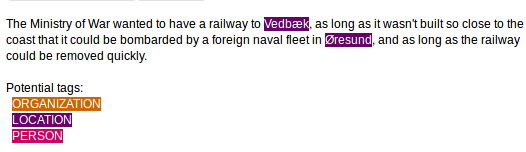
\includegraphics[width=\textwidth]{images/sample_tagging.png}
\end{figure}

The input that was given to the NER tagger was the concatenation of title, summary (as provided by \url{euvsdisinfo}), keywords, and the meta tags content scraped from each individual site.

\subsection{Facebook likes}
The initial dataset, provides only a uniformly weighted list of debunked news cases. In order to provide different weights to the articles in any future visualization, each source URL in the dataset was looked up via facebooks open graph API. The result of the API lookup was a mapping for each source article to a number of likes on facebook, in the case that the information was ever shared on facebook. In \cref{fig:fetch_likes} is seen the essential part of the python code used for fetching the number of likes of each url. The function {\texttt get\_shares} takes as argument a url and returns dictionary of the response from Facebook's API.

\begin{figure}[H]
\caption{Fetching facebook likes for each source URL}
\label{fig:fetch_likes}
\begin{python}
def get_shares(url):
    enc_url = encode(url)
    access_token = get_access_token()
    fields = "og_object{engagement}"
    api_endpoint = "https://graph.facebook.com/v2.11/%s?fields=%s&access_token=%s"
    return requests.get(api_endpoint % (enc_url, fields, access_token)).json()
\end{python}
\end{figure}

\section{Results}
In this section findings findings and results achieved through the process described in the previous section will be presented.

\subsection{Overview}
The resulting dataset from the previous section includes $17$ columns as can be seen in \cref{tab:resulting_dataset}.
\begin{table}[H]
\caption{Resulting columns in the dataset}
\label{tab:resulting_dataset}
\begin{tabularx}{\textwidth}{| l | X |}
    \hline
    {\bf Column name} & {\bf Description} \\ \hline
    {\texttt issue} & The issue number refers to the review the case was published in as given by \href{https://www.euvsdisinfo.eu}{euvsdisinfo.eu}.\\ \hline 
    {\texttt date} & The date the case was reported.\\ \hline
    {\texttt outlet} & The outlet that published the information.\\ \hline
    {\texttt language} & The language the information is provided in.\\ \hline
    {\texttt origin} & Origin of the story, this is sometimes a satirical piece from a different country.\\ \hline
    {\texttt reported by} & The person or organisation who reported the case.\\ \hline
    {\texttt keywords} & Keywords describing the published piece of information.\\ \hline
    {\texttt source} & The URL to the original story, this is not always present i.e. if the source is an interview.\\ \hline
    {\texttt title} & The title of the debunked information.\\ \hline
    {\texttt summary} & The summary of the information that was debunked.\\ \hline
    {\texttt disproof} & The reasoning for \url{euvsdisinfo} to flag the information as dishonest.\\ \hline
    {\texttt metatags} & The types of metatags that included information from the original source during scraping.\\ \hline
    {\texttt metatags\_content} & The content of the metatags that was scraped from the original source.\\ \hline
    {\texttt locations} & Any locations found by the NER tagger.\\ \hline
    {\texttt misc} & Miscellaneously tagged words or phrases tagged by the Stanford NER model. \\ \hline
    {\texttt people} & Recognized names of people by the NER tagger.\\ \hline
    {\texttt likes} & Number of facebook likes registered to the source URL, if any.\\ \hline
\end{tabularx}
\end{table}

The last $6$ columns of \cref{tab:resulting_dataset} are additions to the initial dataset acquired from \href{https://www.euvsdisinfo.eu}{euvsdisinfo.eu}, namely: {\texttt metatags}, {\texttt metatags\_content}, {\texttt locations}, {\texttt misc}, {\texttt people}, and {\texttt likes}.
% \\\\
% The fact that the {\texttt metatags} that were used for scraping content, was included in the final dataset proved 
% The fact that the {\texttt metatags} that were used for scraping content, was included in the final dataset proved interesting later on, as it allowed inspection of which metatags were commonly used. However, the more interesting finding came from the fact that there were no incidents were the metatag for {\texttt author} was included. Now, because of the attempt to reduce duplicate information, it is not possible to conclude whether this was due to content of an {\texttt author} already being included in the scraped data, or if it in reality was missing. However, the fact that no cases included the {\texttt author} tag makes it an interesting aspect to have explored further. However, due to time constraints and for the reason that such investigation would require to rescrape the information, this particular finding was not explored further.
\\\\
In \cref{fig:articles_over_time} is seen the number of articles per date over the period of time that the campaign has been reviewing news information. As seen from the figure, the spread of articles reported over the period remains roughly similar. The graph was created using rawgraphs.io\cite{Mauri:2017:RVP:3125571.3125585}. 
\begin{figure}[H]
    \caption{Articles over time}
    \label{fig:articles_over_time}
    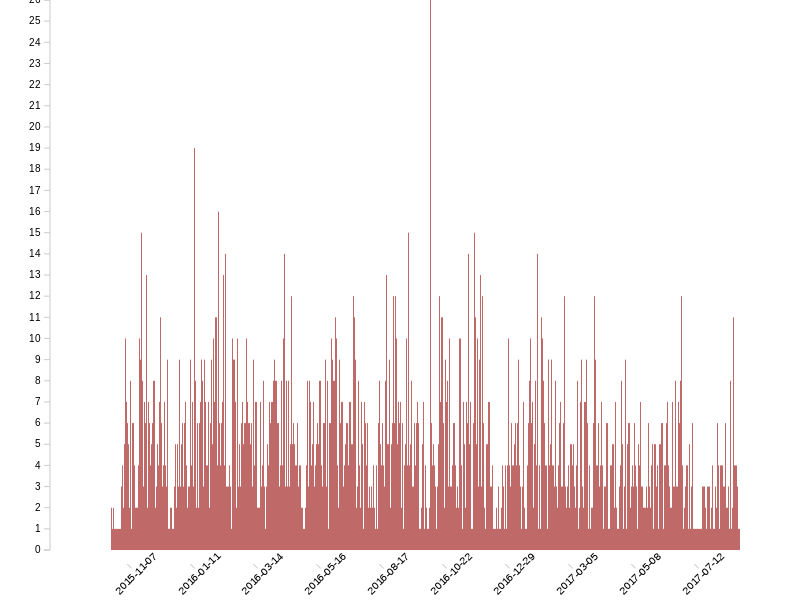
\includegraphics[width=\textwidth]{images/articles_per_date.png}
\end{figure}

As seen in \cref{fig:articles_over_time}, there is a spike in the middle, on 16th october 2016. The spike is largely due to one russian twitter account: {\texttt Vremya pokazhet} that accounted for 10 of the 26 reported cases on that day.


\subsection{Victims and perpetrators}
In this section, the focus will be on the findings that could be of interest towards the initial objective of trying to identify victims and perpertrators in terms of fakenews.
\subsubsection{Locations}
The most mentioned location is, expectedly, Ukraine. Equally unsurprising is the most frequent language, russian, given the focus of the task force behind the campaign on pro-Kremlin news. The top 5 mentioned locations and the 5 most frequent languages is seen in \cref{tab:top5}.
\begin{figure}[H]
\caption{5 most frequent languages and top 5 mentioned locations}
\label{tab:top5}
\centering
\begin{tabular}{l | l}
        \begin{tabular}{l | r}
        {\bf language} & {\bf \% of articles} \\ \hline
            Russian     &   55 \\
            Czech       &   16 \\
            English     &   9 \\
            Slovak      &   2 \\
            Georgian    &   2 \\
        \end{tabular} &
        \begin{tabular}{l | r }
        {\bf location} & {\bf \% of articles} \\ \hline
            Ukraine &   27 \\
            Russia  &   23 \\
            USA     &   21 \\
            Europe  &   8  \\
            Syria   &   5  \\ 
        \end{tabular} \\
    \end{tabular}
\end{figure}

% \subsubsection{Locations}
In general the NER tagger performed well, only $426$ of the $3071$ cases did not have any locations tagged. A sample of the articles tagged is shown in \cref{fig:article_title_lang_loc}. The articles shown were chosen based on having the shortest titles in the dataset, simply because they would be easilier presented while still illustrating the performance of the NER tagger. As can be seen from \cref{fig:article_title_lang_loc}, most sources have recognizable locations which seems intuitively correct given the title. However, at least one in these samples, have falsely tagged locations such as {\texttt PravdaReport}, and the word {\texttt Having}. Since measuring such false positives and equally false negatives, cannot be done quantitatively, this inspection has only been done manually on similar samples. However, it is safe to say that the tagged locations cannot be taken for granted as there will be noise in terms of falsely tagged locations. With that in mind, it can serve as a way of depicting the general pattern of locations named in the disinformation sources.

\begin{figure}[H]
\caption{Sample of cases shown by their title, language and locations}
\label{fig:article_title_lang_loc}
\begin{tabular}{l | l | l }
        {\bf title } & {\bf language } & {\bf locations }\\ \hline
        % Russia never met with the AfD & Russian & Russia \\
        Crimea decided its own fate & Russian & Crimea,Russia,China,India \\
        Ukraine is a neo-Nazi state & Russian & Ukraine,West \\
        NATO is encircling Russia. & Czech & Russia \\
        Ukraine is governed by Nazis. & Russian & Ukraine \\
        Sweden wants to leave the EU. & Spain & Sweden \\
        Georgia is a US colony. & Georgian & Georgia,US \\
        Ukraine has a Nazi identity. & Russian & Ukraine \\
        Ukraine is a part of Russia. & Russian & Ukraine,Russia \\
        Savchenko is a US spy. & Russian & US \\
        Nazis control Ukraine. & Russian & Ukraine \\
        NATO kills Serbian children. & English & PravdaReport,West,Russia,Having,\\
                                     &         & Syria,russia,Serbia,Yugoslavia \\
        Ukraine is governed by nazis. & Russian & Ukraine \\
        All Ukraine is Russia. & Russian & Ukraine,Russia \\
    \end{tabular}
\end{figure}

\subsubsection{People}
The NER tagger also tagged names of people being mentioned in the input, given to it. Filtering these tags for mentioning of {\it Hitler} as well as keywords such as {\it nazi} revealed a pattern of sentiment in the news. The number of articles including one or both of the words, including derivations of the two, was 137 articles. 68\% of those articles were written in russian and 38\% were both written in russian and mentioned Ukraine. 
\\\\
Another finding when looking at the most mentioned names, according to the NER tagger, the name Yekaterina Strizhenova, appears above both Vladimir Putin and Petro Poroshenko, and with some margin. Yekaterina Strizhenova, who appears by her name spelled in cyrillic as seen in \cref{fig:most_mentioned_people}, is a hostess of a TV show called {\it Good Morning} on russian Channel One \cite{good_morning_russia_host}.
\begin{table}[H]
\caption{Most frequently mentioned names}
\label{fig:most_mentioned_people}
\centering
\begin{tabular}{l r}
    {\bf Name} & {\bf Number of appearances} \\ \hline
    Екатерина Стриженова &   68 \\
    Vladimir Putin   & 39 \\
    Petro Poroshenko & 35 \\
\end{tabular}
\end{table} 
% Interestingly, when looking at the most mentioned people appears, above Hitler and Poroshenko, a russian name,. A hostess of a TV show called {\it Good Morning} on russian Channel One.

% \begin{table}[H]
%     \begin{tabular}{l l l l }
% \end{table} 

\subsection{Reporters}
% In this section the findings regarding how reporters listed as having reported the cases to the campaign are distributed.
% \\\\ 
An interesting aspect appears when looking at the values in the {\texttt reported by} column. More than $\frac{1}{3}$ of the cases has been reported by either of two journalists: Pavel Spirin (780 cases) and Oleksandr Nykonorov (379 cases). In third is the European think-tank \href{http://europeanvalues.net/kremlinwatch}{European Values}. Disregarding possible duplicates in the naming of reporting providers, only 33 entities have reported more than 10 cases out of 193 unique entity names. This is an important aspect to consider, besides the focus of the campaign, when considering skewness in the dataset. Oleksandr Nykonorov appears to be a Ukrainian journalist, while the European Values think-tank is an NGO based in the Czech Republic.

\subsection{Considering Facebook likes}
From the 3070 cases the sources averaged roughly 1200 likes on Facebook, although most likes were given to very few articles, as seen in \cref{fig:likes_per_article}. Interestingly, approximately 27\% of all the news sources were either never shared or not liked on Facebook at all.

\begin{figure}[H]
\caption{Likes per article, created using rawgraphs \cite{Mauri:2017:RVP:3125571.3125585}}
\label{fig:likes_per_article}
\centering
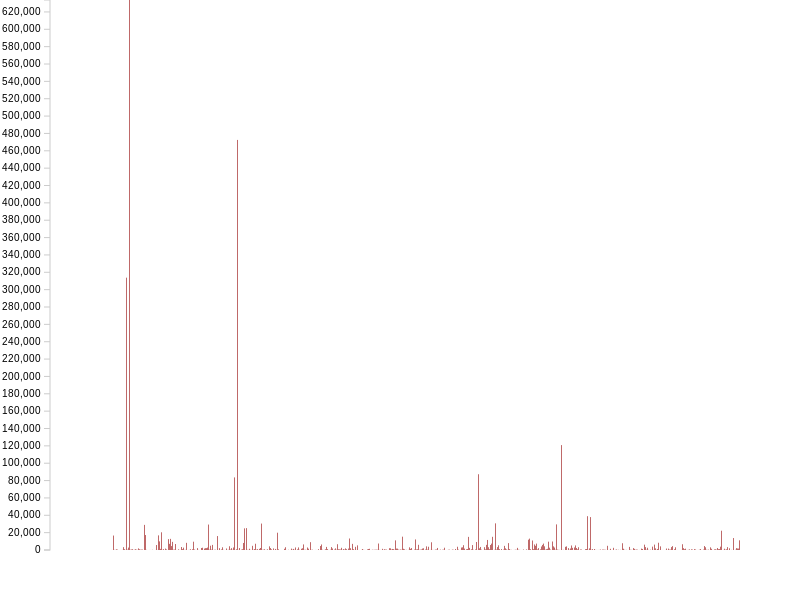
\includegraphics[width=.8\textwidth]{images/articles_vs_likes.png}
\end{figure}

For the purpose of allowing more visual inspection of the dataset, an online visualization was created using \href{https://d3js.org}{d3} and inspired from Mike Bostocks example seen in \url{https://bl.ocks.org/mbostock/4063582}. The visualization uses either of 3 predefined columns from the dataset: {\texttt Language}, {\texttt reported by}, and {\texttt outlet} to create a treemap visualization. While the treemap may not be optimal for all purposes, it goes a long way of showing the earlier mentioned proportionality within the dataset such as the number of articles reported by indivual entitites. In \cref{fig:viz4kidz} is seen a screenshot of this visualization, the screenshot shows the treemap of the number of articles reported by each person or organization within the different languages. The labels are hard to capture, since, for visual clarity, only entities having reported more than 50 articles have a label. On the website other labels will show upon mouse hovering. The colors as well as the squares represents the selected groupings in order. In the case of \cref{fig:viz4kidz} the color is determined by the language. The dark blue, which is most dominant, represents russian. The size of each square in \cref{fig:viz4kidz} indicates the number of articles each entity has reported. The website with the visualization is available as a proof-of-concept at \url{http://k4lk.dk:3000}, for which medium the visualization was optimized for.
% The colors represents different languages, the dark blue, which is most present, represents russian. Each square represents how many articles an entity has reported. As an example it can be seen that for russian, Pavel Spirin has reported the most cases.
\begin{figure}[H]
\caption{Screenshot of the treemap visualization using grouped data by {\texttt language} and then {\texttt reported by} column}
\label{fig:viz4kidz}
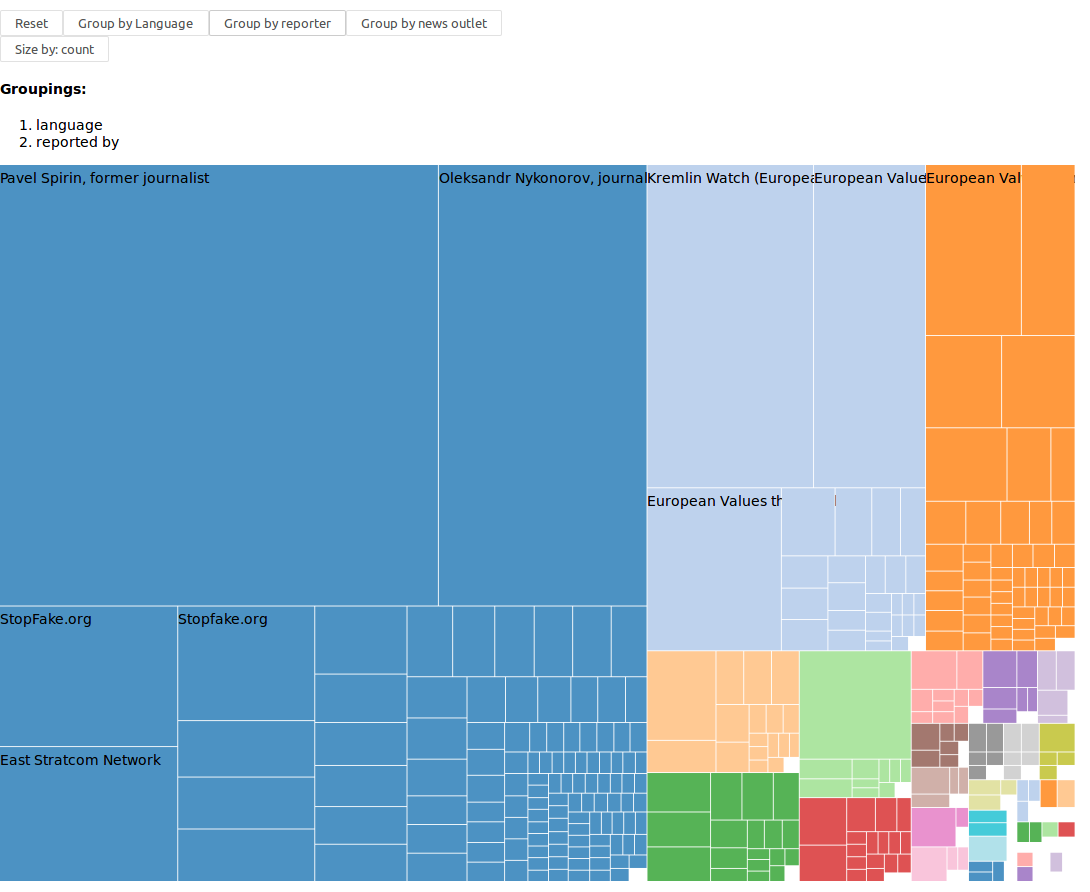
\includegraphics[width=\textwidth]{images/reportedBy_perLanguage_sizeByCount.png}
\end{figure}

Another possible option for the user is to set the size of the squares not by number of cases, but after how many facebook likes each source url accumulated. For information that has not been shared on facebook, the number of likes defaults to zero. 
\\\\
In \cref{fig:lang_bycountorlikes} is shown two more screenshot illustrating how the view changes depending on what units the size of the squares is measured in. In \cref{subfig:lang_count} the size is set by the number of articles for each language, while in \cref{subfig:lang_likes} the size is set to the number of likes for each language. Even though, the visualization is hard to convey to a report format, as it was intended for the web, it can be infered that the view changes drastically in relation to what units is used for sizes. As such, \cref{subfig:lang_count} shows the dominating language is russian when measuring by number of articles, this is aligned with earlier stated properties of the dataset, see \cref{tab:top5}. However, in \cref{subfig:lang_likes}, when looking at the number of Facebook likes in connection to each language, english emerges as largest of them all. Also, from \cref{subfig:lang_likes} it is seen that each language as distinguished by the colors, consists of a few remarkably larger boxes which is to say that a few articles succeeds in gaining a tremendous traction on social media, invariant of the language it is published in.   
 \begin{figure}[H]
\caption{Cases grouped by language and sized either by number of cases, or accumulated likes of each case.}
\label{fig:lang_bycountorlikes}
\begin{subfigure}{\textwidth}
\caption{Language by number of articles}
\label{subfig:lang_count}
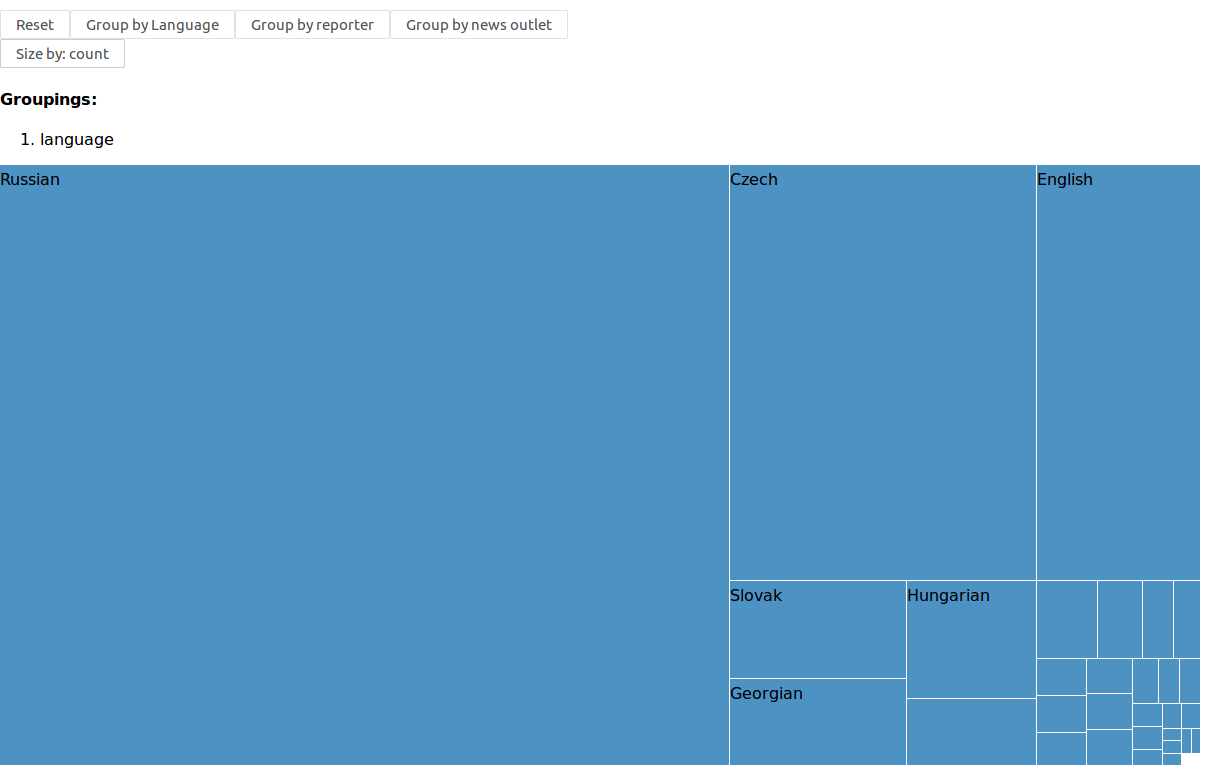
\includegraphics[width=\textwidth]{images/lang_by_count.png}
\end{subfigure}
\begin{subfigure}{\textwidth}
\caption{Language by amount of likes}
\label{subfig:lang_likes}
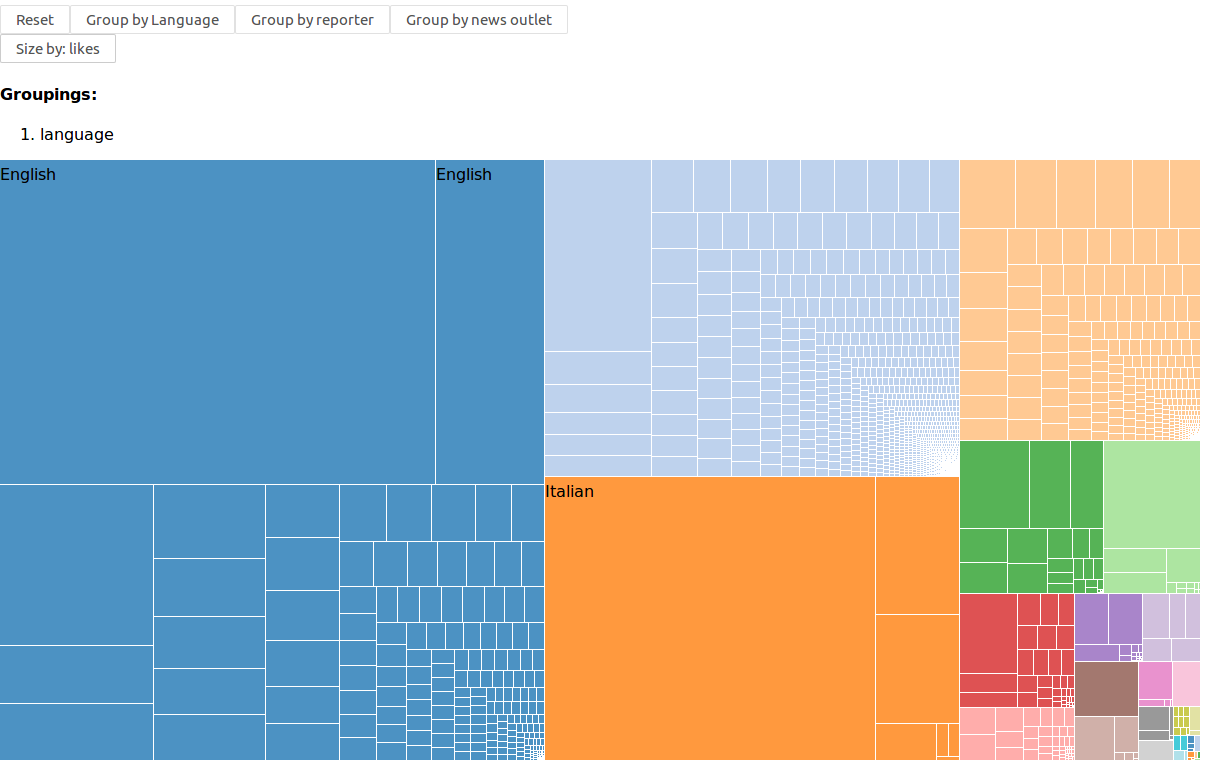
\includegraphics[width=\textwidth]{images/lang_by_likes.png}
\end{subfigure}
\end{figure}

\section{Discussion}

Throughout the project gradually expanded dataset from the initial dataset from \href{https://euvsdisinfo}{euvsdisinfo.eu}, the overall steps can be boiled down to the following 3: 
\begin{itemize}
\item Scraping content from HTML tags related to SEO
\item Extracting named entitites using Stanford NLP
\item Like count for each source URL via Facebook's OpenGraph API 
\end{itemize}
\subsection{Interpreting fake news as attacks}
From this dataset there are may possibilities in terms of visualizations, for this reason it perhaps lends itself best to a dynamic visualization as the proof-of-concept website illustrated in \cref{fig:viz4kidz}. This is further indicated by how the view changes drastically when weighting by likes compared to number of articles.
\\\\
However, in terms of depicting who the perpetrators are, it is very difficult to extract automatically, let alone illustrate. In other areas, say IT security, for a typical visualization by an intrusion detection systems, the roles are clear and consise. A malicious agent scans or otherwise attempts to compromise the system the that the intrusion detection system is guarding. Thereby, the field of intrusion detection easily translate to so called attack maps.\\
Even with respect to "narrative battles" as seen in terms of the Ukranian crisis regarding Crimea, where these distinguished roles certainly exists, it is a non trivial problem to extract this information. This inspite of \href{https://euvsdisinfo}{euvsdisinfo.eu} providing as structured data as has been the case. The reason is that these sort of 'attacks' will take on many shapes and forms and to an extend will blend with regular media. Another factor, is the contextless extraction of the NER tagger. An example of this is seen in of the filtered news articles as shown earlier, where an article is written in russian mentioning Putin, Poroshenko, and Adolf Hitler. A manual consideration would come to the conclusion that the inclusion of Hitler, is only related to the ukrainean president, given the language and origin of the story.
% are not mentioned in the same light.
However, a more automated process of interpretation may come to the false conclusion that both Putin and Poroshenko are victims of such fakenews.

\subsection{Improving awareness}
In any case, despite the difficulties, different views seems an adamant requirement to standing a chance in communicating what fakenews is and how it works. The dataset from \href{https://euvsdisinfo}{euvsdisinfo.eu} has obvious limitations regarding a full picture of fakenews, since it is by definition focused on false news surrounding a Kremlin agenda and because the number of cases is skewed regarding the people reporting them. The fact that a russian TV hostess shows up as the most mentioned name might mean that her TV show is a common source of misinformation. But with respect to the few people who are reporting most of the cases, it may also mean that there exists a disproportionate focus on that TV show in particular. Although, for this specific instance, it seems that Channel One is already identified as an important media for the russian governments ``information warfare'' \cite{the_narrative_battle}. Regardless, this example stresses the importance of having more views not only in terms of including different ways of inspecting the data, as in visualizations, but also to include more sources. Perhaps with respect to including other repositories, but it seems an a equally good option, when the campaign already exists and have established ways for entitites to report cases, that more sources are involved with reporting the cases of fakenews to the campaign.

\subsection{Limitations of the campaign}
In light of the difficulties of visualizations the question arises of how to purposefully make use of the debunked articles in a way that promotes the objective of the campaign: to counter the false knowledge provided by fakenews. The campaign itself posts reviews regularly to their Facebook and Twitter accounts regarding their debunked news cases. This seems their main approach while maintaining a list of all the cases on their website. The same list that was ultimately scraped for usage in this project. However, the list of cases, while constituting a form of repository of debunked fakenews, does not provide any form of API or a download button. This seems counterintuitive to the decision of maintaining it in the first place. A download button seems a must while an API would be an optimal approach for allowing others to further extend the reach of the information that was, from an EU perspective, thought to be vital enough for a task force led campaign to be established.
\\\\
On this note, another question that arose throughout this project concerns how it was even meant to reach the people who would need the debunked news to begin with. Not providing an easy access to their collected dataset other than the view they present themselves on their website, leaves it almost entirely to be distributed through their channels on socialmedia. However, this approach taps into the very same problematics that regular news is already experiencing. The body of information is too vast for anyone to gain a complete overview of. Seeing as how fakenews is already optimized to exploit all the key parameters to win the battle for attention within this context, this approach seems a lost cause.
\\\\
A major challenge of relying on socialmedia to inform of cases of fakenews is that its distribution becomes controlled by the very same filter bubbles that the fakenews is already thriving in. That is, this approach may never manage to bridge between disjointed filter bubbles which is necessary to reach the audience who were susceptible to buying into the original false knowledge that the campaign later debunks. Instead it is more likely that the people who finds their information via their socialmedia accounts were never targeted with the original content.
\\\\
That these groups of people might be disjointed in terms of the information in its original form and the information after it has been debunked, also proposes a whole other challenge. Looking at how 27\% of the cases were never shared on Facebook or was simply never liked if they were, further suggest that if these groups in fact are disjoint, then the campaign risks exposing the news to an audience who would have otherwise not known of its existence.

\subsection{Going forward}
This section will include discussion points on promising directions moving forward, besides the points already stated about the necessity for easier access to the dataset itself. \\
One of the approaches used in this project that proved very capable was the approach to using metatags for acquiring data from uniquely defined websites in a structured way. The approach is not a novel idea, and in fact it is by definition a method for acquiring structured data, one that is used every day by search engine crawlers. However, it is worth mentioning since it neatly exploits the fact that fakenews is created with the common purpose of being spread. In an online context, being spread is inseparable from SEO. Because of this, the approach proved very reliable.
\\
Furthermore, one specific aspect to this approach that would be interesting to further investigate, is whether missing tags related to the author of the article is a common phenomon among fakenews outlets. Also, to what extend the usage of author related tags deviates from that of mainstream online media outlets. This reflection came later as some of the sources were visited manually and, for non the visited pages, there was never an author specified. Unfortunately, author related tags was not included in the set of metatags as defined in \cref{fig:python_metatags}, and due to time constraints of the project it was not within the scope to rescrape the sources for further exploration.
\\\\
The interest in spreading effectively is so ingrained in how online media works both, for the news outlets but also for the platforms that they get shared on. The reason is their common interest in generating revenue from advertisement. According to an interview with James Williams, a former Google employee of 8 years working on their advertisement products and tools and currently postdoctoral candidate at Oxford Internet Institute's Digital Ethics Lab \cite{jamesfuckingwilliamseveryone}, the threat does not reside in fakenews alone, but in the way business models based on advertisement dominates the distribution of information as a whole. A circumstance that as James Williams sees it, threatens to undermine democracy. Considering this angle, there is certainly a conflict of interest for a platform based on advertisement revenue to limit the amount of fakenews, that as stated earlier, is better at going viral than their authentic counterparts.
\\\\
Furthermore, the approach of providing debunking information, implicitly assumes that free will determines the consumption of this information. However, as James Williams propose, even if the link the user clicks, is by their own choice, the chance of that click happening was never let up to the user. Putting this idea into perspective, at the other end of every individuals usage of socialmedia platforms is an entire research and development apparatus that has hyperspecialized every aspect of their platform towards engaging the user with the content they present. Engagement that is not meant to enable the individuals values and goals in life, but instead feeds into the shortsighted desires in all of us, systematically {\it stealing our attention} \cite{jamesfuckingwilliamseveryone}. From the userinterface to the algorithms that determines what content is shown when. The motto of Facebooks newsfeed team comes to mind, and the perception that even if the choice was free, the game was already rigged.
\\\\
To this end, it is interesting to notice that the website \href{https://euvsdisinfo}{euvsdisinfo.eu}, an EU led campaign, perhaps signals an entirely wrong focus when it comes to tackling the problem of fakenews. Instead, as James Williams suggests, it might be a matter of introducing a notion of {\it freedom of chance}, something he sees necessary to introduce in legislation. This perhaps is a circumstance that makes the current era different from historically similar occurences of fakenews. Traditionally, freedom of press and speech has been to ensure that the public had access to information to be able to base their opinions on equal empirical grounds. Today, the information is already there in abundance, however, the chance of what we see is not.
% check if author is ever set...
% , that was ultimately scraped for usage in this project. Th
%%%%%%%%%%%%%%%%%%%%%%%%%%%%%%%%%%%%% ALL OLD DISCUSSION POINTS: 
% In terms of visualization there are many possibilities, however, perhaps just as many limitations. One such limitation is in regards of an initial vague
% Visualizations are difficult as they easily become misrepresentative of the dataset, this is especially true for the domain of fakenews. One example is to consider the cases as attacks by a perpetrator on another vicim, where the roles could be countries or news outlets. However, even as the news outlets, the perpetrator, is provided as part of the data from \href{https://euvsdisinfo}{euvsdisinfo.eu}, then it is hard to automize the extraction of what country is the victim. Often it will be seemingly obvious who the victim is, based on the location and the title or summary of the information. An example of such is russian articles that mentions Ukraine while the NER tagger has recognized the two people mentioned: Adolf Hitler and Petro Poroshenko. \\
% However, more often it will be a russian article mentioning two locations: Russia and Ukraine. In such a case it is much more difficult to automize a ruleset of what mentioned country is the actual victim. The reason is that no context is given as to how the locations are being mentioned, so even if an article mentions Russia in a very different light than how it mentions Ukraine, then that context is lost when only the location is extracted, and through a visualization based on this information, both will look like the victim.
% \\\\
% Furthermore, the dataset itself introduces a lot of biases that if not handled carefully might itself promote a false view of the world to the reader. The fact that the \href{https://euvsdisinfo.eu}{euvsdisinfo.eu} was started in 2015 which correlates with the war in Crimea, and the fact that the campaign already focuses on pro Kremlin news stories, will risk overrepresenting russian news articles with respect to the true population of fakenews articles. This is especially important if as to not present these data as representative of the state of fakenews in the world. The same is true for the campaign itself. When debunking news stories that was never shared on social media in the first place, there is a risk of helping the misinformation more than countering it, simply by giving it publicity that it would never have received otherwise. Even if that publicity is negative, it might be more in the interest of the original outlet than simply not having any attention.
% \\\\
% That attention is important is stressed by the fact that the majority of news outlets that were online, had optimized for search engines. Their objective to be as shareable as possible, since they will want their information to spread in order to be effective, by definition makes these websites easily available to crawl and scrape in a structured, reliable way. At least as reliable as webscraping goes. 
% %Even if the set of articles as a whole, is unstructured, simply because each website is very different.
% \\ 
% In this project the attempt to extract information about people and locations that were mentioned in the online articles, worked well using the metatags provided for search engines. The lack of context the words appeared in, made it hard to automize any interpreting visualization. However, it is still interesting without a layer of interpretation to be able to look at the distribution of locations as it provides a perspective on how the focus on Russia manifests itself in the dataset.
% \\\\
% % Possibly move this part to the `'Results`' section:
% The aspect of disproportionality is also interesting in regards to how these cases are presented on the campaign website. All cases as illustrated in \cref{fig:cases} is shown with a uniform importance. However, as seen when requesting the likes via the facebook API for each URL, it becomes clear, that the distribution of likes is very different from this uniform presentation. Whether or not likes is a good measure of impact, the perspective is arguably different when sizing the treemap using the likes of each case, instead of just counting each case. The difference is visually inspectable through the online visualization, \url{http://k4lk.dk:3000}. In \cref{fig:lang_bycountorlikes} is seen a screenshot of each of these two cases. The figures shows the cases grouped by the language they were published in. However, as can be seen in \cref{subfig:lang_count}, the by far most present language in terms of information cases, is russian, but if the same view is measured in number of likes, seen in \cref{subfig:lang_likes}, then english accumulates more than double the amount of likes as the second most liked russian languaged sources (light blue). In \cref{subfig:lang_likes} each square represents an article, thereby it can be seen that a few specific cases dominates in terms of accumulating likes. A few specific cases being exponentially more liked than others, can be seen from the visualization as a pattern across all languages.
% % simple sentiment using hitler etc.
% % similarly, the combination of title, language, and locations could be interesting:
% % the focus on pro-kremlin news together with the Crimea crisis is probably the reason why most mentioned location is Ukraine
% % problem making an attack map, since locations are given no context
% % structured/unstructured tension

%
%%%%%%%%%%%%%%%%%%%%%%%%%%%% END OF OLD DISCUSSION POINTS %%%%%%%%%%%%%%%%%%%%%%%%%%%%%%%%%%%%%%%%%%%%%%%%%%%%
\section{Conclusion}
In order to be able to better counter the impact of fakenews, we need a better understanding of the nature of fakenews. In this project a very small part of the entire body of fakenews was looked at, namely the cases available from \href{https://euvsdisinfo.eu}{euvsdisinfo.eu}.
\\\\
Even though the nature of fakenews makes it nearly impossible to automate the visualization or analysis of fakenews, it is still possible through semi automatic methods, as illustrated in this report. This is only achievable because of resources such as \href{https://euvsdisinfo.eu}{euvsdisinfo.eu}, that makes the metainformation available as collections in a structured manner. In the same way that the various ways information can be debunked, is not achievable in an automatic way, the same can be said for the deeper interpretations of the eventually debunked cases. However, creating a visual perspective goes a long way to better our understanding of underlying patterns. As is true for many complex phenomenons, then no single perspective can provide the whole truth. Similarly, to visualize the underlying patterns in the dataset used for this project, many different views is needed. For this reason, the explorable visualization is a good approach, however the concrete treemap that was the outcome of this project, can only be seen as a limited part of the perspectives needed to understand the phenomenon of fakenews.

\newpage
\bibliographystyle{abbrv}
\bibliography{lit}
\end{document}